
\subsection{exercise 2 - part 1}
\begin{enumerate}
    \item ADLPMM: $f(x) + g(z)$ where $x + Bz = 0$ and $g=0$\\
    with $B = (-A, -A, -D1, -D2)$\\
    $A$ is a matrix with rows equal to $a_i$\\
    $D_1=
    \begin{bmatrix}
        1 & -1 & \cdots & 0 & 0\\
        0 & 1 & -1 & \cdots & 0\\
        \vdots & \vdots & \vdots & \vdots & \vdots\\
        0 & \cdot & 1 & -1 & 0
    \end{bmatrix}
    $ and 
    $D_2=
    \begin{bmatrix}
        0 & 1 & -1 & \cdots & 0 \\
        0 & 0 & 1 & -1 & \cdots \\
        \vdots & \vdots & \vdots & \vdots & \vdots\\
        0 & 0 & \cdot & 1 & -1
    \end{bmatrix}
    $\\\\
    $f(z, w, v, u) = -\sum_{i=1}^m{\log(a_i^T z - b_i)} + \delta_{C:A w \geq b}(w) + \sum_{i=1}^{n-2} \sqrt{v_i^2 + u_i^2}$ \\
    \begin{align*}
        \prox_{\lambda f}(z,w,v,u) = &\left(\frac{z_j-b_j + \sqrt{(z_j-b_j)^2 + 4\lambda}}{2} + b_j\right)^n_{j=1}\\
        & \times \left(\max\{w_j,b_j\}\right)^n_{j=1}\\
        & \times \left((1-\frac{\lambda}{\max\{\sqrt{v_j^2+u_j^2}, \lambda\}})v_j\right)_{j=1}^n\\
        & \times \left((1-\frac{\lambda}{\max\{\sqrt{v_j^2+u_j^2}, \lambda\}})u_j\right)_{j=1}^n
    \end{align*}\\

    $\prox_{\lambda g}(z) = z$\\
    In the algorithm, $\alpha = \rho $ and $\beta = \rho \lambda_{max}(B^T B)$

    \item CP: $f(Qx) + g(x)$ where $g=0$ and $f$ is defined as above\\
    with $Q = (A, A, D1, D2)$\\
    In the algorithm, using Moreau Decomposition, $\prox_{\sigma f^*}(x) = x - \sigma \prox_{\frac{1}{\sigma}f}(\frac{x}{\sigma})$\\
    \begin{figure}[h]
        \centering
        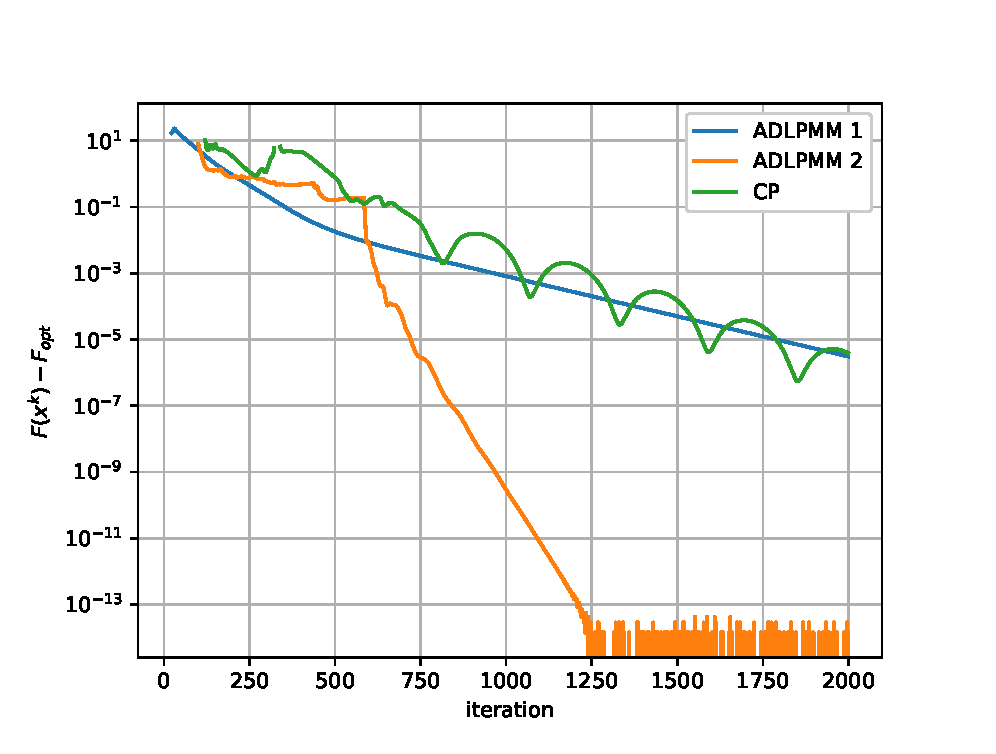
\includegraphics[scale=0.5]{codes/result_images/ex_p3_e2_1_1_results.eps}
        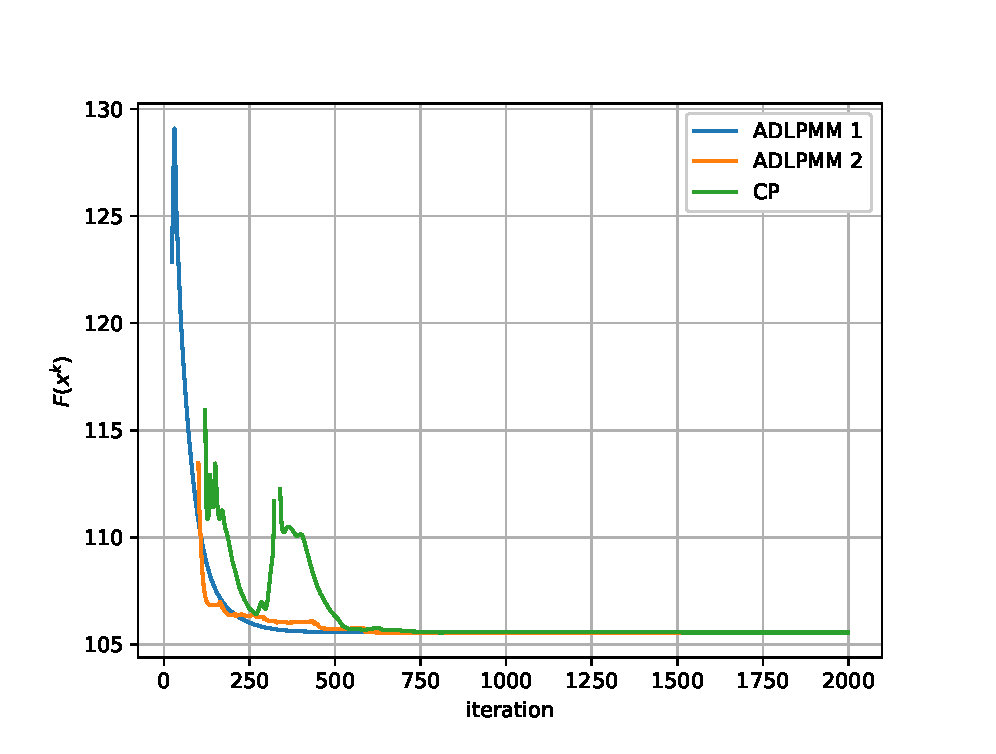
\includegraphics[scale=0.5]{codes/result_images/ex_p3_e2_1_2_results.eps}
        \caption{Part 3, exercise 2, section (c), ADLPMM-1 is with $\rho=1$, ADLPMM-2 is with $\rho=\frac{1}{\|A\|_2}$, and CP is with $\tau=\sigma=\frac{1}{\|A\|_2}$}
        \label{fig:p3e1_1}
    \end{figure}


    \item  Solutions:\\
    ADLPMM 1: $(-5.2156251, 1.41843662, 1.40372643)$\\
    ADLPMM 2: $(-5.2148905, 1.41837664, 1.40349131)$\\
    CP: $(-5.21427958, 1.41827063, 1.40324038)$\\
\end{enumerate}

\subsection{exercise 2 - part 2}
\begin{enumerate}
    \item ACP: $f(Qx) + g(x)$ where $g(x)=\frac{1}{2}\|x\|_2^2$, $Q$ and $f$ is defined as above\\
    $\prox_{\lambda g}(x) = \frac{x}{1+\lambda}$\\
    the strong convexity parameter $\gamma=1$

    \item FDPG: $L_f=\frac{\|Q\|_2^2}{\gamma}$ where $\gamma=1$ is the strong convexity parameter\\
    The update: $u^k = \argmax_u \{\langle u, Q^T w^k \rangle - g(u)\} = Q^T w^k$
    \begin{figure}[ht]
        \centering
        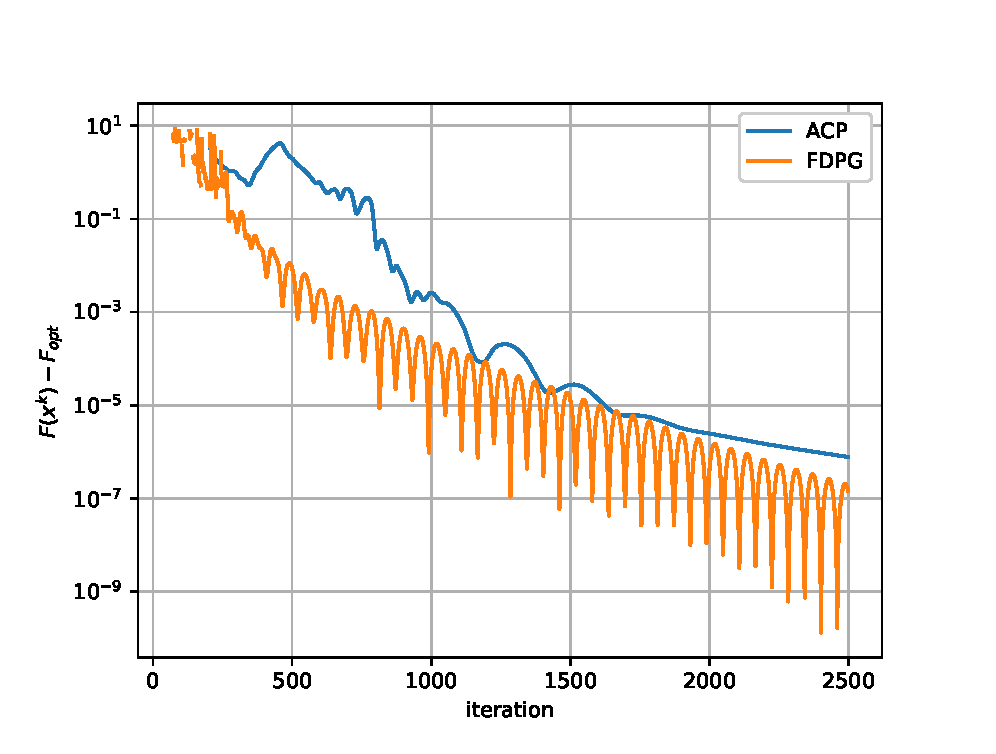
\includegraphics[scale=0.5]{codes/result_images/ex_p3_e2_2_1_results.eps}
        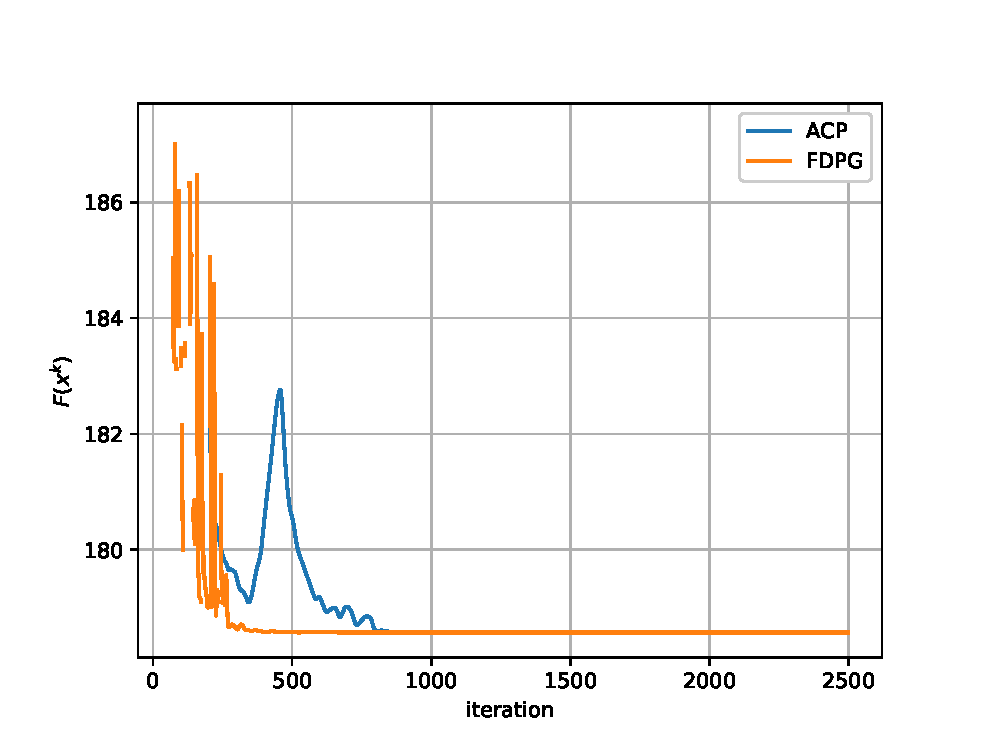
\includegraphics[scale=0.5]{codes/result_images/ex_p3_e2_2_2_results.eps}
        \caption{Part 3, exercise 2, section (e)}
        \label{fig:p3e1_1}
    \end{figure}

    \item Solutions:\\
    ACP: $(-4.26504195, 1.15973671, 1.98584402)$\\
    FDPG: $(-4.264957, 1.1596312, 1.98584261)$
\end{enumerate}
